\chapter{Good design and type safety in Yahtzee - Tom Ellis}
\label{sec:good_design_and_typesafety}


\begin{quotation}
\noindent\textit{\textbf{William Yao:}}

\textit{A worked example of going from a functional, if difficult-to-maintain piece of code, to a design where all the invariants are type-checked and there's no potential crashes to be found.}

\textit{One thing that you should take away from this article is just how much of the refactoring is completely mechanical and required no understanding of the code at all. This is the biggest thing that people are talking about when they say that Haskell is ``easy to maintain'': it's possible to make sweeping changes to your code and improve the design with almost 100\% certainty that it will still work without needing to think about what the code is doing at all.}

\vspace{\baselineskip}

\noindent\textit{Original article:  \cite{good_design_and_type_safety_in_yahtzee}}
\end{quotation}
Mark Dominus wrote an \href{https://blog.plover.com/prog/haskell/type-markers.html}{article asking how to take advantage of Haskell's type safety in a simple dice-rolling simulation function for the game Yahtzee}. He added wrapper types so that one cannot mistakenly apply the function to values that merely have the correct type ``by accident''. He says the result is ``unreadable'' and ``unmaintainable''. It certainly doesn't look nice! I'd claim it's not even of much practical safety benefit (although I suppose that depends on what the rest of the program looks like).

\vspace{\baselineskip}

Mark says:
\begin{quotation}
\noindent \textit{I don't claim this code is any good; I was just hacking around exploring the problem space. But it does do what I wanted.}
\end{quotation} 
But we can't just expect to sprinkle type safety on a bad design and get something good. Type safety and good design are qualities that evolve symbiotically. By using type safety merely to make things safer for our callers we miss out on a host of benefits. Type safety should be used to guide us in the design of our \textit{implementations}, which our callers never see. In fact I would argue that Mark is trying to add type safety in exactly the wrong way.

If there is an interface whose implementation we don't control then all we can do is to slap a type safe wrapper on it and be done with it. That is of some benefit. On the other hand, if we \textit{do} control the implementation then the type safe wrapper specifies invariants that we can take advantage of inside the implementation. They can help us \textit{write} the implementation.

We should build type safe structures and combinators relevant to our domain and implement our solution in terms of those. Likewise we should look at our solution and factor out repeated patterns into type safe structures and combinators relevant to our domain. This is symbiotic evolution!

Type safety and good design proceed hand-in-hand along the road of implementation evolution. Type safety nudges us in the direction of good design and good design nudges us in the direction of type safety. One of the reasons I prefer Haskell to other languages is that the compiler can enforce the type safety end of this bargain. On the other hand, there's no reason a design in Python, say, can't be guided by ``type safety'' in the same sense as a design in Haskell. It's just that the ``type safety'' won't be checked by any tooling and so there's no evolutionary pressure in that direction (Python's recent type annotations notwithstanding).

Let's evolve Mark's program in the direction of good design and see what arises. In this case, as we'll see, I'm not sure there's much to be gained by trying to ``add type safety''. On the other hand, that there is much to be gained by improving the design \textit{guided by} considerations of type safety. The design improvements would apply equally well to an implementation in Python.

I've shown the stages of program evolution as diffs. Sometimes they're easy to read and sometimes they're difficult. If anyone knows how to get diffs to render nicely in Pandoc (perhaps like GitHub renders them) then please please \href{http://web.jaguarpaw.co.uk/~tom/contact/}{contact me}.

\section{Original implementation}

This is the original implementation, before Mark added wrapper types. Most of the refactorings that I will perform are independent of what the implementation actually does; they are simply small changes that are obviously correct. Some are not obviously correct unless you know what the program does, so let's explain that \texttt{allRolls} does the following

\begin{itemize}
\item takes \texttt{DiceState} (a list of dice values and an \texttt{Integer n} of rolls left to perform), and also
\item takes \texttt{DiceChoice} (a choice of which dice to reroll), and
\item returns a list of all the possible rerolls along with an \texttt{Integer} of rolls left to perform.
\end{itemize}
Instead of adding wrapper types let's just try to improve the design and see what happens.

\begin{minted}{haskell}
type DiceChoice = [ Bool ]
type DiceVals   = [ Integer ]
type DiceState = (DiceVals, Integer)

allRolls :: DiceChoice -> DiceState -> [ DiceState ]
allRolls [] ([], n) = [ ([], n-1) ]
allRolls [] _ = undefined
allRolls (chosen:choices) (v:vs, n) =
    allRolls choices (vs, n-1) >>=
        \(roll,_) -> [ (d:roll,  n-1) | d <- rollList ]
          where rollList = if chosen then [v] else [ 1..6 ]

example =
  let diceChoices = [ False, True, True, False, False ]
      diceVals = [ 6, 4, 4, 3, 1 ]
  in mapM_ print $ allRolls diceChoices (diceVals, 2)
\end{minted}

\section{Explain the invariant}

There's a \texttt{undefined} in there. That is always a red flag. In this case undefined occurs when there are dice we could reroll but we haven't specifed whether or not to reroll them: the choice list is too short. Let's explain that in an error message. It communicates better to both the end user of the program and the developer.

We don't need to know what the program does to apply this refactoring but knowing it does give us more confidence that we are doing the right thing.

\begin{figure}[htbp]
 \centering
 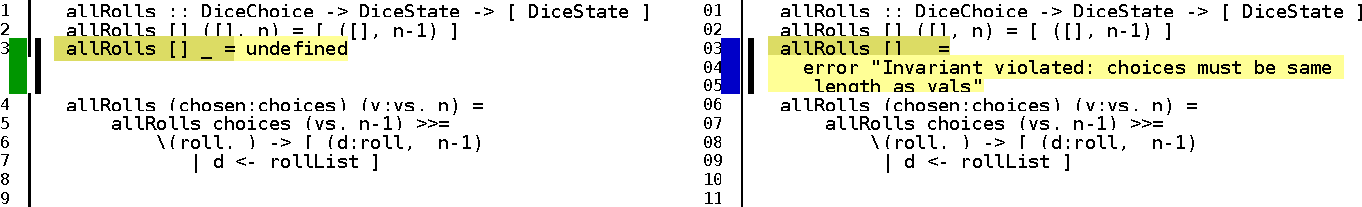
\includegraphics[width=\linewidth]{./pics/diff1.pdf}
 \caption{Explain the invariant}
 \label{fig:diff1}
\end{figure}

\section{Avoid catch-all pattern}

I prefer to have as few overlapping patterns as possible, even ``catch-all'' \texttt{(\_)} patterns. This is a fairly minor change, but let's do it anyway. I think it modestly improves the design.

We don't need to know what the program does to apply this refactoring.

\begin{figure}[htbp]
 \centering
 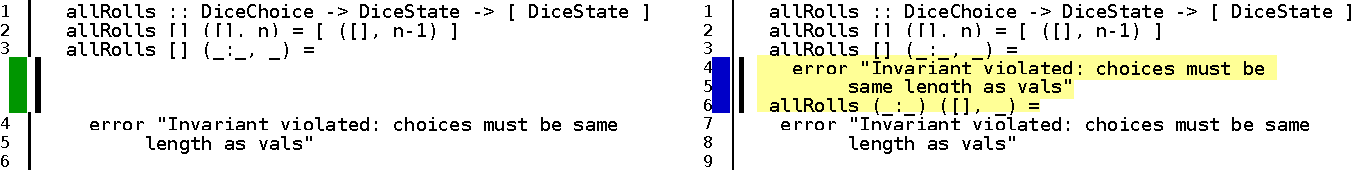
\includegraphics[width=\linewidth]{./pics/diff2.pdf}
 \caption{Avoid catch-all pattern}
 \label{fig:diff2}
\end{figure}

\section{Add another invariant check}

There's actually a missing pattern (which \texttt{-Wall} will pick up). Let's add it. Another modest improvement.

Like with the first invariant check, we don't need to know what the program does to apply this refactoring but knowing it does give us more confidence that we are doing the right thing.

\begin{figure}[htbp]
 \centering
 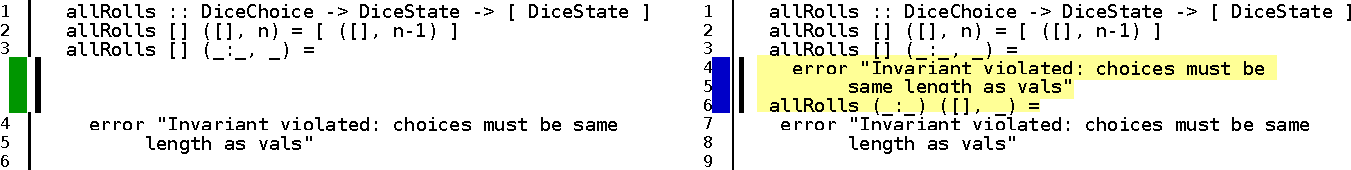
\includegraphics[width=\linewidth]{./pics/diff3.pdf}
 \caption{Add another invariant check}
 \label{fig:diff3}
\end{figure}

\section{Add pop function}

There are two distinct things that \texttt{allRolls} does.

\begin{enumerate}
\item It checks the invariant and if the invariant holds extracts relevant inputs.
\item It runs the algorithm on the relevant inputs.
\end{enumerate}
Let's separate the concerns by adding a \texttt{pop} function that does 1. Note that the interface between \texttt{pop} and \texttt{allRolls} has type safety! Once \texttt{pop} returns, an invalid state is not possible. \texttt{allRolls} does not change, except to pass its argument through \texttt{pop}.

We don't need to know what the program does to apply this refactoring.

\begin{minted}{haskell}
pop :: DiceChoice
    -> DiceVals
    -> Maybe ((Bool, Integer), (DiceChoice, DiceVals))
pop [] [] = Nothing
pop (chosen:choices) (v:vs) = Just ((chosen, v), (choices, vs))
pop (_:_) [] = error "Invariant violated: missing val"
pop [] (_:_) = error "Invariant violated: missing choice"

allRolls :: DiceChoice -> DiceState -> [ DiceState ]
allRolls choices (vs, n) = case pop choices vs of
  Nothing -> [ ([], n-1) ]
  Just ((chosen, v), (choices, vs)) ->
    allRolls choices (vs, n-1) >>=
        \(roll,_) -> [ (d:roll,  n-1) | d <- rollList ]
          where rollList = if chosen then [v] else [ 1..6 ]
\end{minted}


\section{Indicate that a value is unused}


This is the first time we have to apply real thinking to the design process. Weirdly, the $n-1$ argument to the recursive call to \texttt{allRolls} is not used in the final result. The only way I can suggest that one discovers this is to think through how the the code actually works. Unlike the above changes, this is not just a simple refactoring.

Let's indicate that the argument is unused by applying an error instead. In a language without lazy evaluation you might like to apply some nonsense value like -999999999 instead, and check that the results of the function call are not nonsense!

When we run this we don't get a crash, which implies that that argument was indeed not used.

\begin{figure}[htbp]
 \centering
 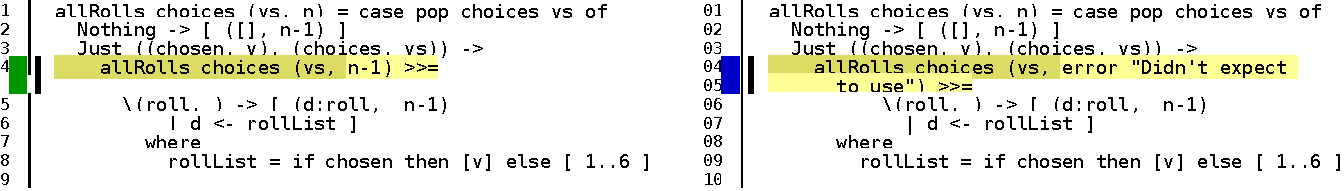
\includegraphics[width=\linewidth]{./pics/diff4.pdf}
 \caption{Indicate that a value is unused}
 \label{fig:diff4}
\end{figure}
           
\section{Prepare to rearrange arguments}


Given the observation above I see no reason to package the \texttt{DiceVals} and the \texttt{Integer} together. Let's prepare to separate them.

We don't need to know what the program does to apply this refactoring. We just have to observe that the \texttt{DiceVals} and the \texttt{Integer} are not really used together.

\begin{figure}[htbp]
 \centering
 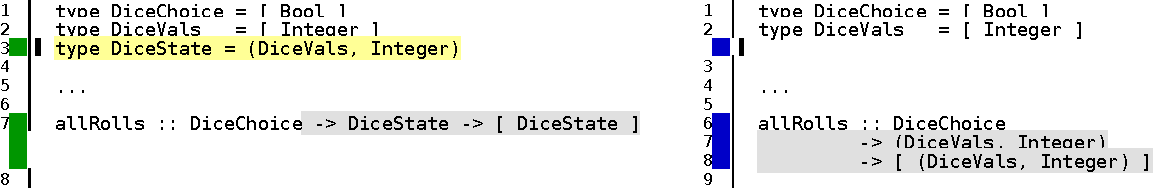
\includegraphics[width=\linewidth]{./pics/diff6.pdf}
 \caption{Prepare to rearrange arguments}
 \label{fig:diff6}
\end{figure}

\section{Rearrange arguments}


Now let's do the separation of the arguments. The size of the diff makes the change seem bigger than it is. It is merely passing two arguments instead of a tuple!

We don't need to know what the program does to apply this refactoring.

\begin{figure}[htbp]
 \centering
 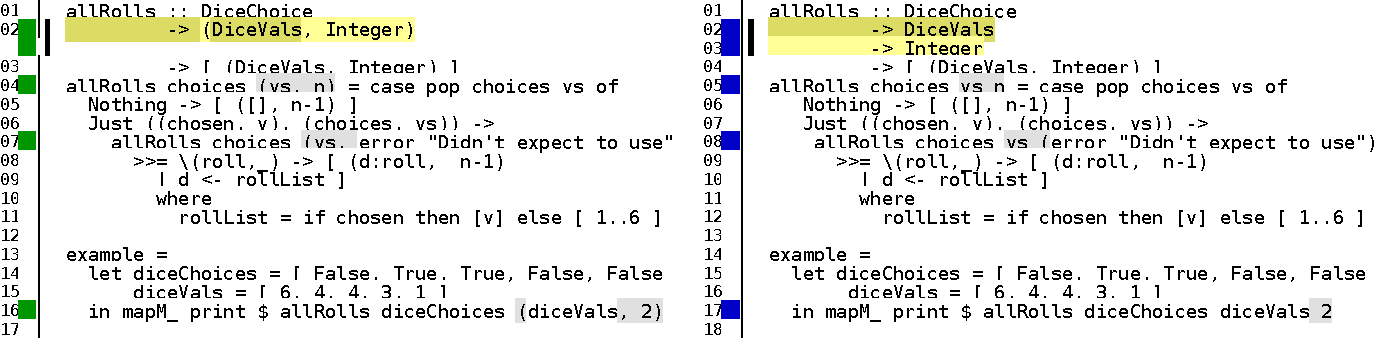
\includegraphics[width=\linewidth]{./pics/diff5.pdf}
 \caption{Rearrange arguments}
 \label{fig:diff5}
\end{figure}

\section{Rearrange arguments further}

Once we have separated \texttt{DiceVals} from the \texttt{Integer} we notice that \texttt{DiceChoice} and \texttt{DiceVals} seem to naturally belong together. Again the diff makes the change look bigger than it is. We're just passing \texttt{DiceChoice} and \texttt{DiceVals} as a tuple rather than two arguments.

We don't need to know what the program does to apply this refactoring.

\begin{figure}[htbp]
 \centering
 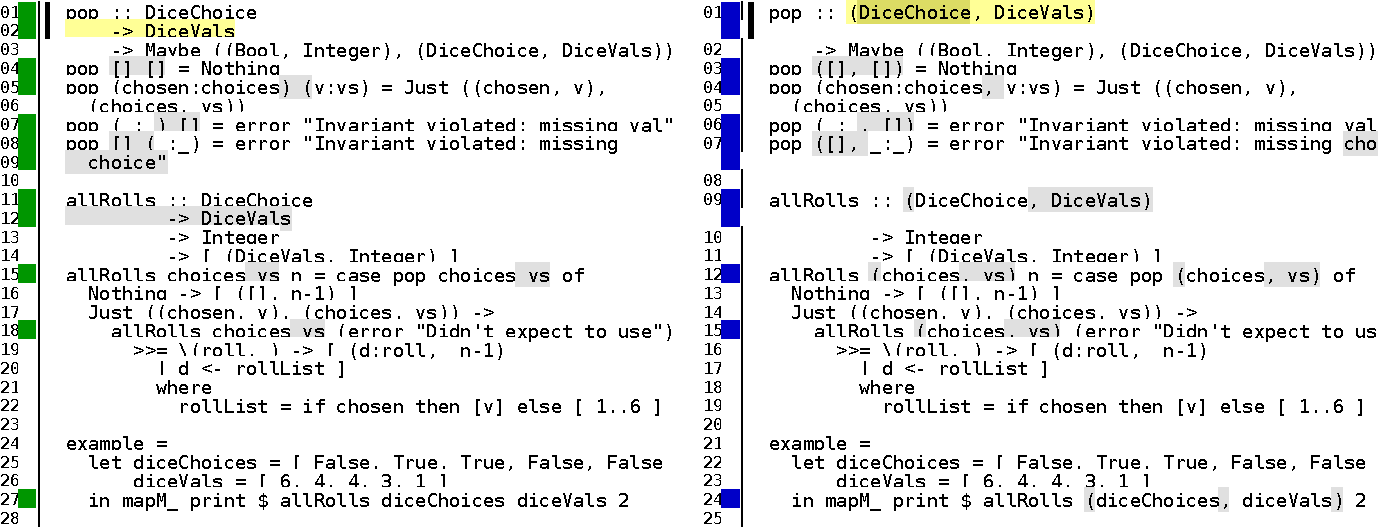
\includegraphics[width=\linewidth]{./pics/diff7.pdf}
 \caption{Rearrange arguments further}
 \label{fig:diff7}
\end{figure}

\section{Avoid unpacking tuple}


We no longer need to unpack the tuple! We don't need to know what the program does to apply this refactoring.

\begin{figure}[htbp]
 \centering
 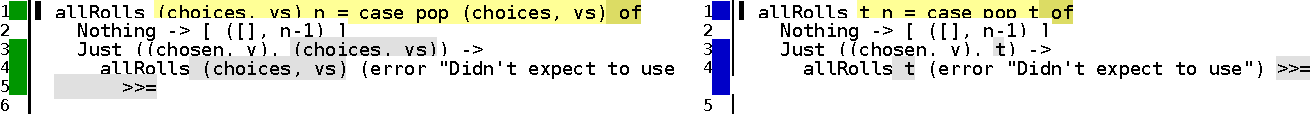
\includegraphics[width=\linewidth]{./pics/diff8.pdf}
 \caption{Avoid unpacking tuple}
 \label{fig:diff8}
\end{figure}

\section{We don't use the Integer. Make this structural.}


Given that we have an unused argument in the recursive call let's see if we can change our design to make this obvious, i.e. make the fact that we don't use it an essential part of the structure of the program, not just a property. In this case it amounts to pairing the rolls with $n-1$ after the bulk of the algorithm (\texttt{allRollsNoN}) has finished.

This is the second time we have to actually analyse how our program works rather than just apply a mechanical translation.

\begin{figure}[htbp]
 \centering
 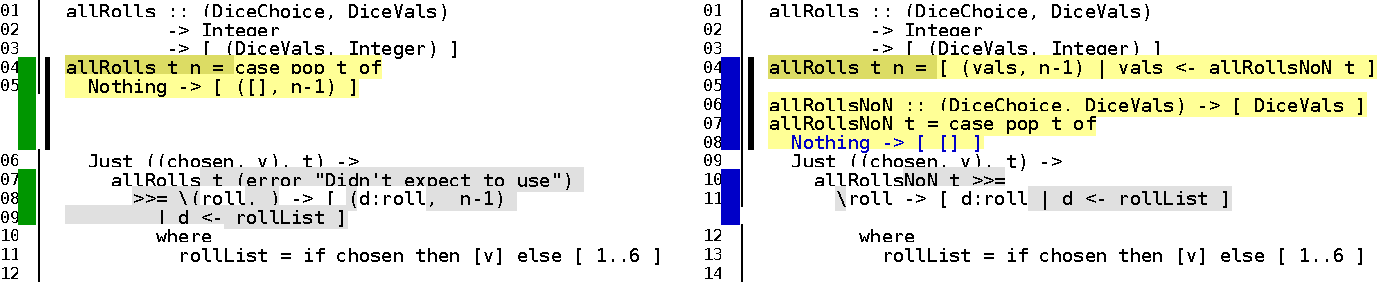
\includegraphics[width=\linewidth]{./pics/diff9.pdf}
 \caption{We don't use the Integer}
 \label{fig:diff9}
\end{figure}

\section{Introduce a type synonym}


Given that \texttt{DiceChoice} and \texttt{DiceVals} seem to belong together let's add a type synonym (\texttt{DiceTurn}) for that.

We don't need to know what the program does to apply this refactoring. We just observe that the pair of things are always used together.

\begin{figure}[htbp]
 \centering
 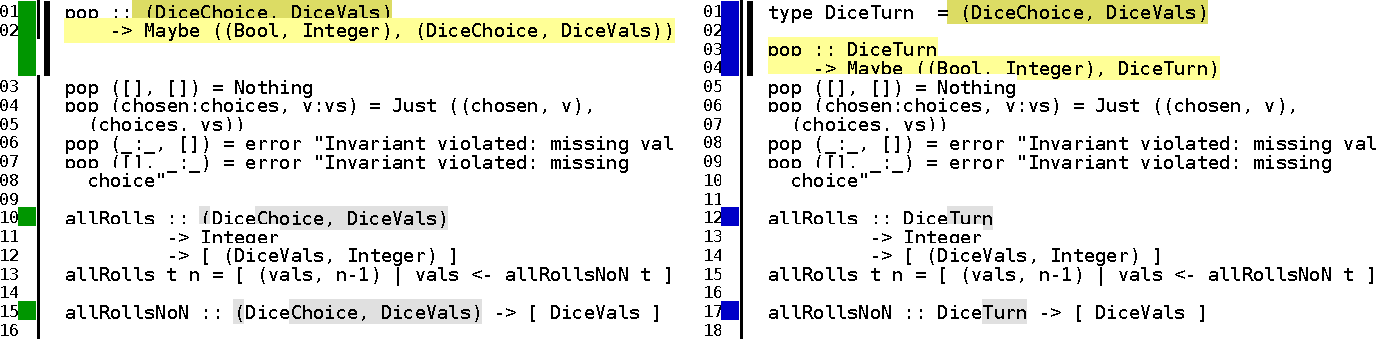
\includegraphics[width=\linewidth]{./pics/diff10.pdf}
 \caption{Introduce a type synonym}
 \label{fig:diff10}
\end{figure}


\section{Make illegal states unrepresentable}


Our invariant is that the number of \texttt{DiceChoices} must be the same as the number of \texttt{DiceVals}. Semantically, we actually want something stronger: each of the \texttt{DiceChoices} corresponds to exactly one of the \texttt{DiceVals}. In my experience this is the single most common non-trival failure to structurally enforce program behaviour (and \href{https://twitter.com/fried_brice/status/1178140883633479680}{I'm not the only one to see it}).

The fix is to put pairs of dice choice and dice vals in the same list! We can entirely remove our invariant check. The invariant is enforced by the type.

Consumers will have to change too but they'll be better off for it! In \texttt{example} I just \texttt{zip}ped the args. It could also be something much better.

\begin{figure}[htbp]
 \centering
 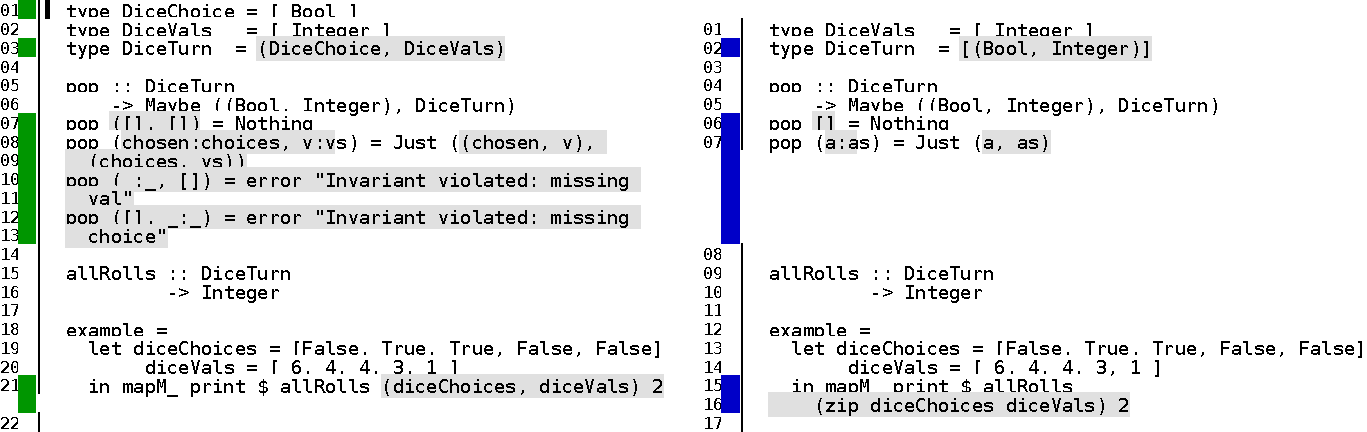
\includegraphics[width=\linewidth]{./pics/diff11.pdf}
 \caption{Make illegal states unrepresentable}
 \label{fig:diff11}
\end{figure}

\section{Use uncons}

Having done that we see that \texttt{pop} is just the standard function ``\texttt{uncons}''. We don't need to know what the program does to apply this refactoring.

\begin{figure}[htbp]
 \centering
 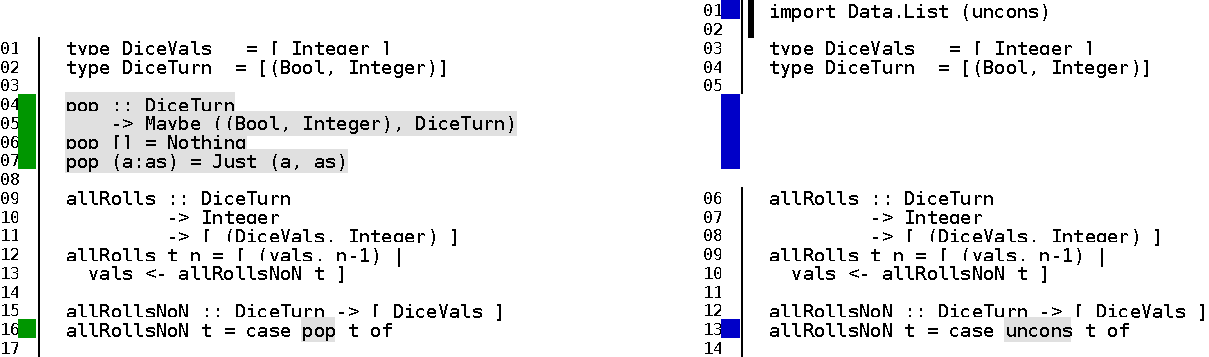
\includegraphics[width=\linewidth]{./pics/diff12.pdf}
 \caption{Use uncons}
 \label{fig:diff12}
\end{figure}

\section{Don't need uncons}


Having said that, we don't actually need \texttt{uncons}. We can just pattern match directly. We don't need to know what the program does to apply this refactoring.

\begin{figure}[htbp]
 \centering
 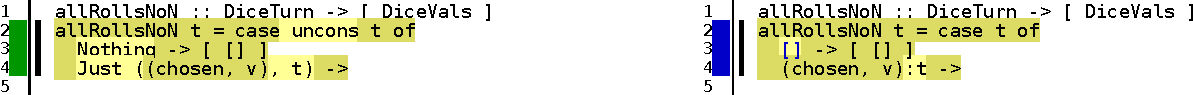
\includegraphics[width=\linewidth]{./pics/diff13.pdf}
 \caption{Don't need uncons}
 \label{fig:diff13}
\end{figure}

\section{Use do notation}

The use of the bind operator (\texttt{>>=}) and list comprehension are not particularly clear. Let's rewrite it to use do notation. (In fact I recommend defaulting to do notation over operators unless there's some compelling readability benefit to using the latter.)

We don't need to know what the program does to apply this refactoring.

\begin{figure}[htbp]
 \centering
 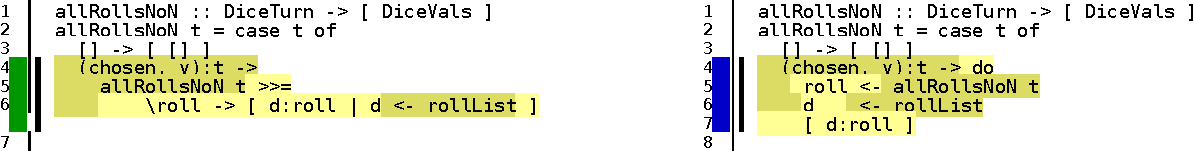
\includegraphics[width=\linewidth]{./pics/diff14.pdf}
 \caption{Use do notation}
 \label{fig:diff14}
\end{figure}


\section{Prepare for \texttt{mapM}}

We can see from the above that what our program does is takes the head of a list, runs recursively on the tail, does something to the head, and then puts it back on the tail. This is a ``map'' operation. Specifically in this case we are mapping in a monad so we use \texttt{mapM}. In modern Haskell you'd use \texttt{traverse}, but I'm going to stick to \texttt{mapM} because \texttt{traverse} does not read so well. (\texttt{traverse} really ought to be called \texttt{mapA} but \href{https://www.reddit.com/r/haskell/comments/68w09h/proposal_to_add_mapa_as_synonym_for_traverse/}{people don't like the idea of that change}.)

In this change we just make the function we are mapping take explicit arguments. We'll switch to use \texttt{mapM} in the next change. 
We don't need to know what the program does to apply this refactoring.

\begin{figure}[htbp]
 \centering
 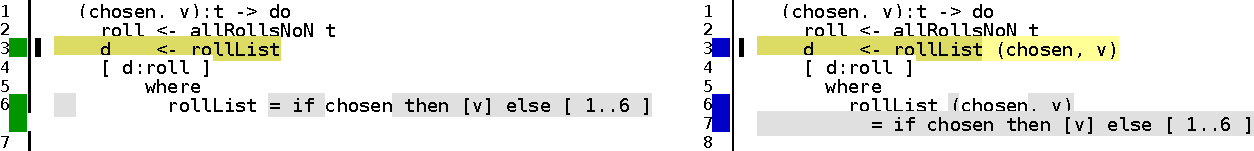
\includegraphics[width=\linewidth]{./pics/diff15.pdf}
 \caption{Prepare for \texttt{mapM}}
 \label{fig:diff15}
\end{figure}


\section{Use \texttt{mapM}}

Now we can just use \texttt{mapM} directly. 
We don't need to know what the program does to apply this refactoring but we do need to know the general concept of ``mapping'' and the specific implementation \texttt{mapM}. Be careful! This particular ``refactoring'' actually reverses the order of effects -- the list of dice rolls will come out in a different order.

\begin{figure}[htbp]
 \centering
 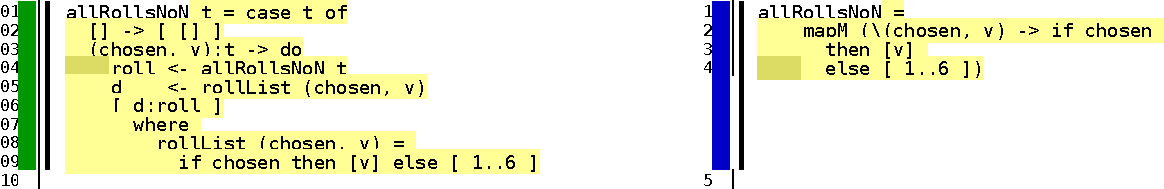
\includegraphics[width=\linewidth]{./pics/diff16.pdf}
 \caption{Use \texttt{mapM}}
 \label{fig:diff16}
\end{figure}


\section{Avoid boolean blindness}


There's ambiguity in the type \texttt{DiceTurn = [(Bool, Integer)]}. Does the \texttt{Bool} refer to whether we keep the dice or to whether we reroll them? There's no way for me to tell without seeing this conditional inside the function:

\begin{minted}{haskell}
if chosen then [v] else [ 1..6 ]
\end{minted}
Ah, so the \texttt{Bool} refers to whether we keep the dice. Perhaps this is written in the documentation somewhere, but why do I believe that the documentation is kept in line with the implementation? I want a single source of truth!

Let's add a type to avoid ``boolean blindness''. The type of \texttt{allRollsBetter} still does not guarantee that the implementation does the right thing with its argument but it does make any deviation glaringly obvious.

We don't need to know what the program does to apply this refactoring. It requires the uncontroversial \texttt{LambdaCase} language extension.

\begin{figure}[htbp]
 \centering
 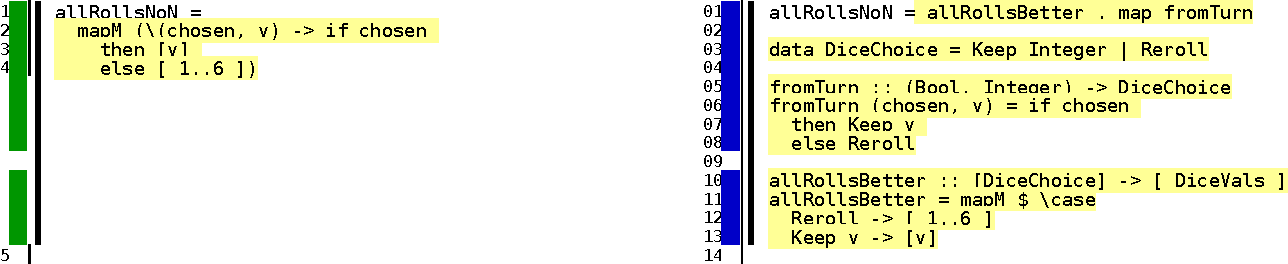
\includegraphics[width=\linewidth]{./pics/diff17.pdf}
 \caption{Avoid boolean blindness}
 \label{fig:diff17}
\end{figure}



\section{Keep the better version}


Let's get rid of all vestiges of the old version. What \texttt{allRolls} does could be done more clearly at the call site. At this point I wouldn't add wrapper types for ``type safety''. The rest of the program might be sufficiently complex that they would help, but they certainly don't add anything in this simple example.

The new version communicates \textit{much} better. We ``map'' over our \texttt{DiceVals} list, that is, apply a function to each element in turn. In this case we're taking advantage of the \texttt{Monad} instance for lists, so we use \texttt{mapM}. The function we map simply says

\begin{itemize}
\item Do we want to \texttt{Reroll}? If so, the possible results are \texttt{[1..6]}  
\item Do we want to \texttt{Keep v}? If so, the possible results are just \texttt{[v]}
\end{itemize}


\begin{minted}{haskell}
{-# LANGUAGE LambdaCase #-}

type DiceVals   = [Integer]
data DiceChoice = Keep Integer | Reroll

allRollsBetter :: [DiceChoice] -> [DiceVals]
allRollsBetter = mapM $ \case
  Reroll -> [1..6]
  Keep v -> [v]

example =
  let diceVals = [ Reroll, Keep 4, Keep 4, Reroll, Reroll ]
  in mapM_ print $ allRollsBetter diceVals
\end{minted}
Look at \texttt{allRollsBetter} in comparison to the original \texttt{allRolls}!

\begin{minted}{haskell}
allRolls :: DiceChoice -> DiceState -> [ DiceState ]
allRolls [] ([], n) = [ ([], n-1) ]
allRolls [] _ = undefined
allRolls (chosen:choices) (v:vs, n) =
    allRolls choices (vs, n-1) >>=
        \(roll,_) -> [ (d:roll,  n-1) | d <- rollList ]
          where rollList = if chosen then [v] else [ 1..6 ]
\end{minted}
How did we end up with something so much clearer? We applied a sequence of transformations to improve the design, almost all of which are applicable in any language. The transformations were partly informed by a notion of ``type safety''. Specifically, we aimed to model our domain using types and functions that make illegal states unrepresentable.

None of this \textit{requires} a language like Haskell. It would be good design in Python as well. One of Python's weaknesses is that it makes dealing with sum types awkward. We would have had to take a slightly different approach for the \texttt{Maybe} returned by \texttt{pop} (probably \texttt{None} or a tuple), the \texttt{DiceChoice} type (probably a pair of classes) and the list monad (probably just a recursive generator function). Ultimately though, the benefit of Haskell is not that it allows us to implement well-typed designs, nor particularly that it forbids us from implementing ill-typed designs. The benefit is that it nudges us away from poorly-typed, poorly-structured designs \textit{and holds our hand as it does so}.








\chapter{Using our brain less in refactoring Yahtzee - Tom Ellis}

\textit{Original article: \cite{using_our_brain_less}}

\vspace{\baselineskip}

\noindent Cameron Gera and Taylor Fausak \href{https://haskellweekly.news/episode/22.html}{produced a podcast} on an article of mine about good design and typesafety (see section \ref{sec:good_design_and_typesafety}) using code from an implementation of the game Yahtzee. The article is about refactoring code to improve design and how that goes hand-in-hand with type safety. Intriguingly, listening to others talk about my article gave me fresh ideas.

At one point in the article we observed that a variable to an argument was unused. Subsequently we removed it. The only justification given that the removal of the argument was valid was that we could convince ourselves that it was unused by looking at the implementation of the function, and that we could insert a run time check.

Hearing Cameron and Taylor talk about the article made me think again. There were only two changes to the code that really relied upon understanding what it does; everything else was mechanical transformation. Both of those changes were to do with the unused argument.

Einstein said ``chalk is cheaper than grey matter''. Can we avoid using ``grey matter'' (our brains) to remove the unused argument, instead just relying on ``chalk'' (mechanical transformations)? The answer is yes! Let's see how to do it.

\section{The starting point}


We start from the ``Add pop function'' stage of the previous article. We've got a suspicion that, although the argument \texttt{n} to \texttt{allRolls} \textit{is} used, the argument $n-1$ to the recursive call is not. How can we transform the code to make that clear?

\begin{minted}{haskell}
type DiceChoice = [ Bool ]
type DiceVals   = [ Integer ]
type DiceState  = (DiceVals, Integer)

pop :: DiceChoice
    -> DiceVals
    -> Maybe ((Bool, Integer), (DiceChoice, DiceVals))
pop [] [] = Nothing
pop (chosen:choices) (v:vs) = Just ((chosen, v), (choices, vs))
pop (_:_) [] = error "Invariant violated: missing val"
pop [] (_:_) = error "Invariant violated: missing choice"

allRolls :: DiceChoice -> DiceState -> [ DiceState ]
allRolls choices (vs, n) = case pop choices vs of
  Nothing -> [ ([], n-1) ]
  Just ((chosen, v), (choices, vs)) ->
    allRolls choices (vs, n-1) >>=
        \(roll,_) -> [ (d:roll,  n-1) | d <- rollList ]
          where rollList = if chosen then [v] else [ 1..6 ]

example =
  let diceChoices = [ False, True, True, False, False ]
      diceVals = [ 6, 4, 4, 3, 1 ]
  in mapM_ print $ allRolls diceChoices (diceVals, 2)
\end{minted}

\section{Use do-notation}


Let's immediately simplify by using do-notation. In the previous article we left this stage until later but given that the recursive call is currently part of a \texttt{>>=} expression let's apply the simplification now.

\begin{minted}{haskell}
allRolls :: DiceChoice -> DiceState -> [ DiceState ]
allRolls choices (vs, n) = case pop choices vs of
  Nothing -> [ ([], n-1) ]
  Just ((chosen, v), (choices, vs)) -> do
    (roll, _) <- allRolls choices (vs, n-1)
    [ (d:roll, n-1) | d <- rollList ]
          where rollList = if chosen then [v] else [ 1..6 ]
\end{minted}


\section{Observe that both branches pair a list with n-1}


If the argument \texttt{n} were not used at all then our job would be much easier. However, it \texttt{is} used, so let's try to separate the place it is used from the place where (we believe) it is not used.

Where is it used? We can see that each branch of the \texttt{case} statement returns a list of tuples where the second element of each tuple is $n-1$. Put another way, each branch produces a list and then maps the ``pair with $n-1$'' function over it.

I'll write the ``pair with n-1'' function as \verb|(, n-1)| (using the \texttt{TupleSections} extension). The usual alternative would be to write \texttt{\\x -> (x, n-1)} but in this article I want to keep things compact.

\begin{figure}[htbp]
 \centering
 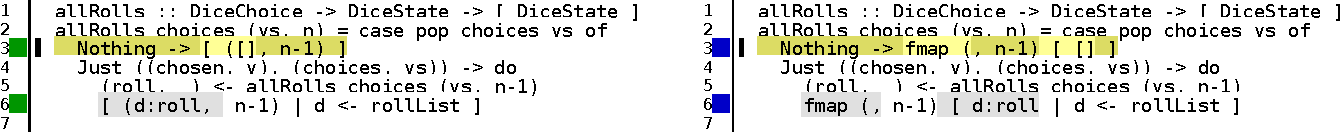
\includegraphics[width=\linewidth]{./pics/diff18.pdf}
 \caption{Observe that both branches pair a list with n-1}
 \label{fig:diff18}
\end{figure}


\section{Lift fmap outside \texttt{do}}


Now \texttt{n} is used, we think, just twice, and in each case to map the ``pair with $n-1$'' function over a list. We've made this duplication obvious but we can't yet remove it. First we have to lift the fmap outside the do. We use the rule that

\begin{minted}{haskell}
do ...
   fmap f e
can be rewritten to

fmap f $ do ...
            e
\end{minted}
Why is this rewriting valid? Informally, a \texttt{do} block is like a procedure, and this rule says that ``applying f and then returning from the procedure'' is the same as ``returning from the procedure and then applying f''. Formally, it can be proved using the monad laws.

This is how the rewriting applies in our case:

\begin{figure}[htbp]
 \centering
 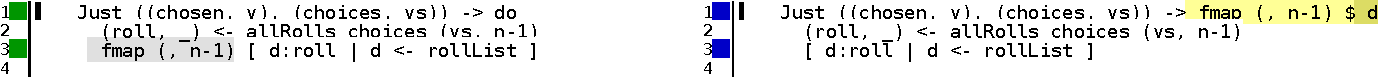
\includegraphics[width=\linewidth]{./pics/diff19.pdf}
 \caption{Lift fmap outside \texttt{do}}
 \label{fig:diff19}
\end{figure}
 
\section{Combine duplicated functions at top level}


Now that both branches of the case statement are \texttt{fmap (, n-1)} of something, we can apply \texttt{fmap (, n-1)} to the overall case statement instead. Specifically, the rule is that we can rewrite

\begin{minted}{haskell}
case x of
    Case1 -> f $ body1
    Case2 -> f $ body2
\end{minted}
to

\begin{minted}{haskell}
f $ case x of
    Case1 -> body1
    Case2 -> body2
\end{minted}
which in our code leads to

\begin{figure}[htbp]
 \centering
 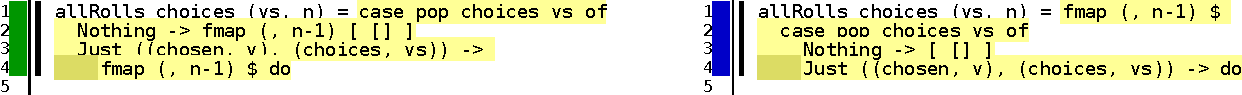
\includegraphics[width=\linewidth]{./pics/diff20.pdf}
 \caption{Lift fmap outside \texttt{do}}
 \label{fig:diff20}
\end{figure}


\section{Split function body into separate function}


We want to carefully separate the parts of the code for which the value of \texttt{n} matters from the parts of the code for which the value of n does not matter. To this end we split the body of \texttt{allRolls} into a separate function called \texttt{allRollsBody}.

\begin{figure}[htbp]
 \centering
 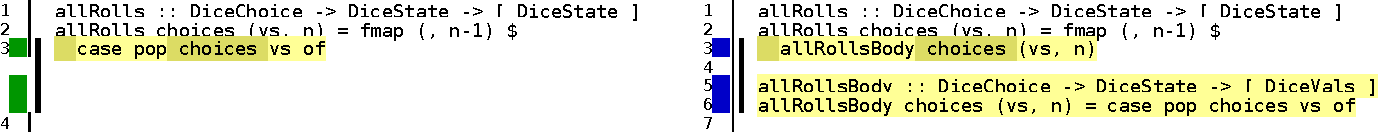
\includegraphics[width=\linewidth]{./pics/diff21.pdf}
 \caption{Split function body into separate function}
 \label{fig:diff21}
\end{figure}


\section{Substitute definition of \texttt{allRolls}}

Now we are in the nice situation that, although we are yet to prove it to our satisfaction, the value of \texttt{allRollsBody} does not depend on its argument n.

However, we've ended up with a pair of mutually recursive functions! That's somewhat unusual. In order to make \texttt{allRollsBody} recurse only on itself we substitute the definition of \texttt{allRolls} back into \texttt{allRollsBody}. Additionally, that makes \texttt{allRolls} not recursive at all.

\begin{figure}[htbp]
 \centering
 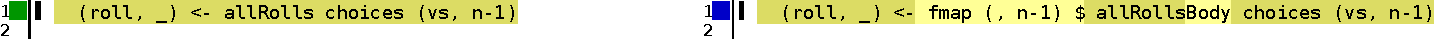
\includegraphics[width=\linewidth]{./pics/diff22.pdf}
 \caption{Substitute definition of \texttt{allRolls}}
 \label{fig:diff22}
\end{figure}


\section{Remove redundant pairing}


We're pairing every element of a list with $n-1$ and then immediately removing it. Let's just avoid the pairing in the first place.

\begin{figure}[htbp]
 \centering
 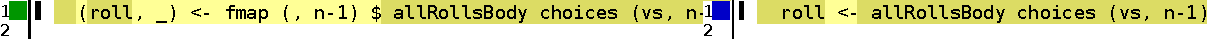
\includegraphics[width=\linewidth]{./pics/diff23.pdf}
 \caption{Remove redundant pairing}
 \label{fig:diff23}
\end{figure}


\section{Generalise type of \texttt{allRollsBody}}


Now the magic happens! Our code currently looks like this.

\begin{minted}{haskell}
allRolls :: DiceChoice -> DiceState -> [ DiceState ]
allRolls choices (vs, n) = fmap (, n-1) $ allRollsBody choices (vs, n)

allRollsBody :: DiceChoice -> DiceState -> [ DiceVals ]
allRollsBody choices (vs, n) = case pop choices vs of
  Nothing -> [ [] ]
  Just ((chosen, v), (choices, vs)) -> do
    roll <- allRollsBody choices (vs, n-1)
    [ d:roll | d <- rollList ]
          where rollList = if chosen then [v] else [ 1..6 ]
\end{minted}
Previously we had to use our brains to spot that the \texttt{Integer} argument to the recursive call was unused. We inserted a run time check to convince ourselves that we were right. Now we have split the original function into two, only one of which contains a recursive call. We can see clearly that the only use for the argument n to \texttt{allRollsBody} is to be modified and passed to the recursive call. The value of that argument is never used in any other way. From that observation alone we are probably satisfied that we can remove it.

In fact we can go one step better. We can make a small change to our code so that we do not even have to inspect the implementation to know that n is unused. The compiler will check the property for us! However, the check is demonstrated in a strange way, and if you're not familiar with it then it will look utterly bizarre.

We generalise the type signature so that the function doesn't just work for an \texttt{Integer} but rather for \textit{any} type of numeric argument \texttt{a}, that is, any type \texttt{a} with an instance of the \texttt{Num} type class.

\begin{minted}{haskell}
allRollsBody :: Num a => DiceChoice -> (DiceVals, a) -> [DiceVals]
\end{minted}
Believe it or not, from this type signature alone, without knowing anything about the implementation, we can conclude that the a argument is not used! How on earth can we conclude that? It's because of the \href{https://en.wikipedia.org/wiki/Parametricity}{parametricity} property enjoyed by Haskell's type system. Basically, the type signature says that the only operations involving type a that \texttt{allRollsBody} can use are the ones from the \texttt{Num} type class. \href{https://www.stackage.org/haddock/lts-13.21/base-4.12.0.0/Prelude.html#t:Num}{Looking at them}, we see that they give us a way to \textit{make} new as from an \texttt{Integer} (\texttt{fromInteger}) and ways to combine as to give other as (\texttt{+}, \texttt{*}, etc.). On the other hand, there is no way that a value of another type can be \textit{created from} an \texttt{a}. Therefore, the only way that an argument of type a could be used to affect the result is if the type variable a appears in the type of the result. The result has type \texttt{[DiceVals]} so it cannot be affected by the argument of type \texttt{a}!

If that seems baffling to you, do not be despondent. Although parametricity is an extremely sophisticated property using it in practice becomes second nature. Haskell programmers use it to great advantage in creating APIs which remain flexible whilst providing strong guarantees via their type signatures.

\section{Remove unused argument}


One way or another, our program transformations have taken us to a place where we feel comfortable removing the \textit{Integer} argument without having to think too hard about the justification. We can inspect the body and see that the argument is not used in a way that can affect the result or we can use parametricity to deduce the same thing. Either way we can remove it.

\begin{minted}{haskell}
allRolls :: DiceChoice -> DiceState -> [ DiceState ]
allRolls choices (vs, n) = fmap (, n-1) $ allRollsBody choices vs

allRollsBody :: DiceChoice -> DiceVals -> [ DiceVals ]
allRollsBody choices vs = case pop choices vs of
  Nothing -> [ [] ]
  Just ((chosen, v), (choices, vs)) -> do
    roll <- allRollsBody choices vs
    [ d:roll | d <- rollList ]
          where rollList = if chosen then [v] else [ 1..6 ]
\end{minted}


\section{Conclusion}


In the earlier article I said that ``the only way I can suggest that one discovers [that the argument is unused] is to think through how the the code actually works\ldots this is not just a simple refactoring''. I was wrong! There is a small sequence of simple transformations that improve the code whilst at the same time taking us to a place where we easily see that the argument is unused. For the latter either we use a small amount of brainpower to inspect the implementation or we take advantage of parametricity. This is great! We want to save as much brainpower as possible for the really hard problems.

A small amount of Haskell knowledge was required but that is because the code is written in Haskell. Other languages will have their own particular constructs and equivalent transformations, although if they lack \texttt{case} statements and expression-valued blocks the transformations might appear a bit more clunky. The only typed-functional-language-specific concept in this article is parametricity. In this small example we were happy to just inspect the body of the function. Parametricity really shines in more complicated codebases where unrelated, opaque, pieces of functionality are being combined.








